
\documentclass[tikz]{standalone}

\begin{document}

% adjust the [scale=X] value to make it 
% the size you want.

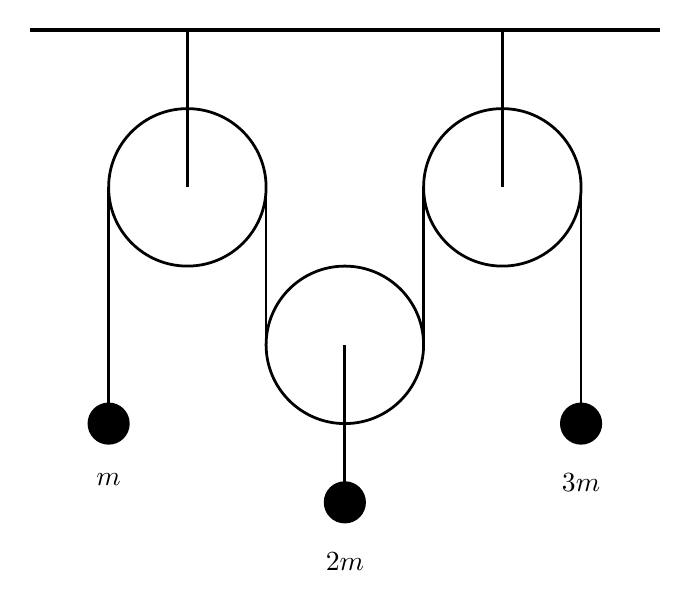
\begin{tikzpicture}[scale=10,line width=1pt]
% ceiling
\draw [ultra thick] (0,0) -- (.8,0);
% left pulley
\draw (.2,-.2) circle [radius=0.1];
\draw (.2,0) -- (.2,-.2);
% left mass
\draw (.1,-.2) -- (.1,-.5);
\draw [fill=black] (.1,-.5) circle [radius=0.025];
\node [below] at (.1,-.55) {$m$};
% second pully
\draw (.3,-.2) -- (.3,-.4);
\draw (.4,-.4) circle [radius=0.1];
% second mass
\draw (.4,-.4) -- (.4,-.6);
\draw [fill=black] (.4,-.6) circle [radius=0.025];
\node [below] at (.4,-.65) {$2m$};
% third pully
\draw (.5,-.2) -- (.5,-.4);
\draw (.6,-.2) circle [radius=0.1];
\draw (.6,0) -- (.6,-.2);
% third mass
\draw (.7,-.2) -- (.7,-.5);
\draw [fill=black] (.7,-.5) circle [radius=0.025];
\node [below] at (.7,-.55) {$3m$};
\end{tikzpicture}


\end{document}
